\documentclass{llncs}
\let\ifpddf\relax
%%%%%%%%%%%%%%%%%%%%%%%%%%%%%%%%%%%%%%%%%%%%%%%%%%%%%%%%%%%
%% package sillabazione italiana e uso lettere accentate
\usepackage[latin1]{inputenc}
\usepackage[english]{babel}
\usepackage[T1]{fontenc}

%%%%%%%%%%%%%%%%%%%%%%%%%%%%%%%%%%%%%%%%%%%%%%%%%%%%%%%%%%%%%

\usepackage{url}
\usepackage{xspace}

\makeatletter
%%%%%%%%%%%%%%%%%%%%%%%%%%%%%% User specified LaTeX commands.
\usepackage{manifest}

\makeatother


%%%%%%%
 \newif\ifpdf
 \ifx\pdfoutput\undefined
 \pdffalse % we are not running PDFLaTeX
 \else
 \pdfoutput=1 % we are running PDFLaTeX
 \pdftrue
 \fi
%%%%%%%
 \ifpdf
 \usepackage[pdftex]{graphicx}
 \else
 \usepackage{graphicx}
 \fi
%%%%%%%%%%%%%%%
 \ifpdf
 \DeclareGraphicsExtensions{.pdf, .jpg, .tif}
 \else
 \DeclareGraphicsExtensions{.eps, .jpg}
 \fi
%%%%%%%%%%%%%%%

\newcommand{\java}{\textsf{Java}}
\newcommand{\contact}{\emph{Contact}}
\newcommand{\corecl}{\texttt{corecl}}
\newcommand{\medcl}{\texttt{medcl}}
\newcommand{\msgcl}{\texttt{msgcl}}
\newcommand{\android}{\texttt{Android}}
\newcommand{\dsl}{\texttt{DSL}}
\newcommand{\jazz}{\texttt{Jazz}}
\newcommand{\rtc}{\texttt{RTC}}
\newcommand{\ide}{\texttt{Contact-ide}}
\newcommand{\xtext}{\texttt{XText}}
\newcommand{\xpand}{\texttt{Xpand}}
\newcommand{\xtend}{\texttt{Xtend}}
\newcommand{\pojo}{\texttt{POJO}}
\newcommand{\junit}{\texttt{JUnit}}

\newcommand{\action}[1]{\texttt{#1}\xspace}
\newcommand{\code}[1]{{\small{\texttt{#1}}}\xspace}
\newcommand{\codescript}[1]{{\scriptsize{\texttt{#1}}}\xspace}

% Cross-referencing
\newcommand{\labelsec}[1]{\label{sec:#1}}
\newcommand{\xs}[1]{\sectionname~\ref{sec:#1}}
\newcommand{\xsp}[1]{\sectionname~\ref{sec:#1} \onpagename~\pageref{sec:#1}}
\newcommand{\labelssec}[1]{\label{ssec:#1}}
\newcommand{\xss}[1]{\subsectionname~\ref{ssec:#1}}
\newcommand{\xssp}[1]{\subsectionname~\ref{ssec:#1} \onpagename~\pageref{ssec:#1}}
\newcommand{\labelsssec}[1]{\label{sssec:#1}}
\newcommand{\xsss}[1]{\subsectionname~\ref{sssec:#1}}
\newcommand{\xsssp}[1]{\subsectionname~\ref{sssec:#1} \onpagename~\pageref{sssec:#1}}
\newcommand{\labelfig}[1]{\label{fig:#1}}
\newcommand{\xf}[1]{\figurename~\ref{fig:#1}}
\newcommand{\xfp}[1]{\figurename~\ref{fig:#1} \onpagename~\pageref{fig:#1}}
\newcommand{\labeltab}[1]{\label{tab:#1}}
\newcommand{\xt}[1]{\tablename~\ref{tab:#1}}
\newcommand{\xtp}[1]{\tablename~\ref{tab:#1} \onpagename~\pageref{tab:#1}}
% Category Names
\newcommand{\sectionname}{Section}
\newcommand{\subsectionname}{Subsection}
\newcommand{\sectionsname}{Sections}
\newcommand{\subsectionsname}{Subsections}
\newcommand{\secname}{\sectionname}
\newcommand{\ssecname}{\subsectionname}
\newcommand{\secsname}{\sectionsname}
\newcommand{\ssecsname}{\subsectionsname}
\newcommand{\onpagename}{on page}

\newcommand{\xauthA}{NameA StudentA }
\newcommand{\xauthB}{NameB StudentB}
\newcommand{\xauthC}{NameC StudentC}
\newcommand{\xfaculty}{II Faculty of Engineering}
\newcommand{\xunibo}{Alma Mater Studiorum -- University of Bologna}
\newcommand{\xaddrBO}{viale Risorgimento 2}
\newcommand{\xaddrCE}{via Venezia 52}
\newcommand{\xcityBO}{40136 Bologna, Italy}
\newcommand{\xcityCE}{47023 Cesena, Italy}

%
% Comments
%
%%% \newcommand{\todo}[1]{\bf{TODO:}\emph{#1}}


\begin{document}

\title{Ingegneria dei Sistemi Software\\ Approfondimento \\ \footnotesize Terza Parte}

% \author{\xauthA \and \xauthB}
\author{Beatrice Mezzapesa, Alessia Papini, Lorenzo Pontellini}

\institute{%
%%%  \xunibo\\\xaddrCE, \xcityCE\\\email{\{nameA.studentA, nameB.studentB\}@studio.unibo.it}
  \xunibo\\\xaddrCE, \xcityCE\\\email\{beatrice.mezzapesa, alessia.papini, lorenzo.pontellini\}@studio.unibo.it
}

\maketitle

%% \begin{abstract}
%% \footnotesize
%%This a Latex template to be used for the reports of Software Engineering.
%%\keywords{Software engineering, managed software development, reports, ....}
%%\end{abstract}

%%% \sloppy

\section{Problem Analysis}

Riproponiamo alcuni concetti relativi all'analisi del problema presentati nella precedente relazione\footnote{Ingegneria dei Sistemi Software A differential drive Robot Seconda Parte}, utili contestualizzare questo lavoro:
\begin{quotation}\itshape
	"Visto il contesto nel quale ci si pone, le problematiche identificate hanno portato, come citato all'interno dell'analisi dei requisiti, alla definizione di una serie di concetti per le varie modalit� di esecuzione delle azioni. Occorre identificare una modalit� che ci permetta di astrarre dallo specifico problema in gioco (ovvero quello dei robot) e che ci consenta di definire una soluzione generale alla problematica, sfruttando il robot come approccio, definendo i concetti validi anche per future fasi evolutive del progetto. I requisiti ci portano a riconoscere una serie di problematiche delle quali ci andremo ad occupare: definizioni di azioni sincrone/asicrone ed azioni interrompibili.\\
	Ponendoci nel contesto di esempio, il robot deve essere sensibile ad alcuni cambiamenti che potranno avvenire nell'ambiente circostante nel quale � situato. Occorre, quindi, definire la gestione di questi cambiamenti in modo che durante l'esecuzione delle azioni previste, nel caso di rilevamento di un cambiamento, il robot possa reagire di conseguenza. In particolare si vuole fare in modo che l'azione intrapresa dal robot si blocchi e si possano eseguire azioni alternative, al termine di queste sar� necessario valutare se continuare o meno con l'esecuzione precedente che include le azioni gi� pianificate. Da qui in avanti viene definito \textbf{piano} come sequenza di azioni.\\
	Cos� facendo occorre definire, dato un robot, tutti i cambiamenti ai quali dev'essere in grado di reagire, descrivendo i comportamenti da avere in ogni situazione e le modalit� di controllo che permettano di fare una valutazione sullo stato di avanzamento dell'azione corrente intrapresa dal robot.
	Inoltre � necessario riconoscere quando un'azione � giunta al termine in modo da controllare lo stato dell'azione ed eventualmente proseguire con la successiva.\\
	La base di partenza per noi � l'astrazione di classe \textbf{BaseRobot} il quale tramite apposito metodo ha la possibilit� di eseguire azioni tramite l'uso di appositi attuatori, all'interno del mondo reale. Legata alla problematica identificata, sorge inoltre il problema di specificare la tipologia di azione da utilizzare all'interno del contesto in esame dato che questa, avr� effetti sul controllo del robot stesso e sul comportamento dell'architettura logica creata a valle.\\
	Si vogliono fissare le definizioni relative alle possibili azioni utilizzate all'interno del contesto del problema appena definito:
	\begin{itemize}\itshape
		\item 	\textbf{Azione sincrona}: si considera un'esecuzione sincrona quando questa viene concretizzata e occorre attendere la terminazione della stessa per poter restituire il controllo al chiamante.
		
		\item 	\textbf{Azione asincrona}: si definisce un'esecuzione asincrona quando questa pu� essere eseguita senza che il chiamante debba attendere la fine dell'esecuzione dato che il controllo viene immediatamente restituito al chiamante.
	\end{itemize}
\end{quotation}

\section{Abstraction Gap}

L'implementazione di quanto descritto precedentemente pu� essere realizzata utilizzando il linguaggio Java, seguendo questo approccio per� non si � in grado di esprimere ad un sufficiente livello di astrazione le tematiche sopra citate e si nota come il dislivello dal punto di vista tecnologico sarebbe troppo ampio per essere colmato in un unico step computazionale, comportando inoltre un'elevato dispendio di tempo.\\
Per ovviare a questo, puntando a rendere pi� semplice la fase implementativa, si decide di sfruttare un'infrastruttura composta da una serie di framework quali: \textbf{QActor} e \textbf{QEvent} proposta nel corso di ?Ingegneria dei Sistemi Software?. Di seguito verrano proposti i concetti fondamentali alla base di tale infrastruttura utili per un'utilizzo ottimale della stessa.\\
QActors � un framework custom utile a mostrare come i progettisti affrontano l'analisi, la progettazione e l'implementazione di sistemi software utilizzando uno stile a message-passing piuttosto che un stile tradizionale basato sugli oggetti. Un QActor � un'entit� attiva che ha lo scopo di eseguire le operazioni di base, quali la ricezione e l'invio di un messaggio, ma pu� anche eseguire un comportamento espresso da un piano, sequenza di azioni/attivit� che hanno un tempo finito per essere eseguite. Questo tipo di modello computazionale potr� essere considerato come assodato per le future implementazioni del problema.
I QActors sono stati utilizzati anche nella prima fase di progetto, pur non essendo strettamente necessari in un sistema concentrato che non ha l'esigenza di considerare la comunicazione attraverso la rete. In particolare come base di partenza si � utilizzata l'entit� RobotActor, che deriva da QActor, e permette l'interazione con il BaseRobot.
Nella seconda fase invece, il contesto da prendere in considerazione � distribuito, in quanto � necessario interagire con il robot per interrompere un'azione, anche in questo caso sar� utilizzata l'entit� RobotActor esteso con la possibilit� di ricevere comandi inviati dalla console remota oppure dal browser. Possiamo, quindi, considerare come primo modello per gestire la comunicazione quello a message-passing. In questo caso, per�, eseguendo un'azione di una durata prefissata non saremo in grado di interromperla in alcun modo (in quanto questo modello non � proattivo/reattivo).\\
Prendendo in considerazione la possibilit� di gestire le azioni eseguite dal robot come un automa a stati finiti e considerando il contesto distribuito nel quale ci troviamo, quindi la presenza della rete, per poter gestire i cambiamenti ai quali il robot deve reagire � necessario introdurre il concetto di Evento e pi� precisamente QEvent. 
QEvent � un framework che permette l'implementazione di sistemi software eternogenei in grado di adottare un modello event-driven. Un evento � un'informazione che viene emessa da una sorgente, che pu� essere esterna nel caso in cui la sorgente sia fisica come la console remota o interna nel caso in cui la sorgente sia un componente software come il robot.\\ 
Questo ci permette di definire che il cambiamento che permette di eseguire la transizione da uno stato all'altro dell'automa pu� essere identificato come un evento. In questo modo si vuole ottenere una entit� reattiva che nel momento in cui esegue un'azione possa comunque essere sensibile a determinati "cambiamenti". Infatti, supponendo di essere in uno stato in cui viene eseguita una determinata azione, il robot si mantiene reattivo e nel momento in cui riceve un particolare evento � in grado transitare in un determinato stato che permetta la
gestione dell'evento stesso.
In particolare, con questa modellazione, si � in grado di definire un evento che viene lanciato al termine dell?esecuzione di un azione sincrona/asincrona. Ovviamente per un particolare stato possono essere definiti pi� eventi ai quali il robot dev'essere sensibile ed altrettante transizioni di stato che permettano di gestirli. In un contesto generale, quando viene ricevuto un evento di "halt", che provoca una transizione di stato, esso viene gestito eseguendo un piano alternativo e fermando l?azione eseguita in precedenza. Nel caso del contesto specifico questo non � necessario in quanto, l'esecuzione di una nuova azione da parte del robot, interrompe/termina automaticamente quella precedente.
Ogni azione eseguita dal robot verr�, quindi, modellata come automa a stati finiti con tante transizioni in diversi stati, quanti saranno gli eventi che potranno essere ricevuti. Per poter realizzare un'azione che durante la sua esecuzione possa essere interrotta, si ha la necessit� di un'entit� distinta che si occupi di percepire e reagire gli eventuali eventi ricevuti, ovvero un \textbf{EventHandler}. A sua volta quest'entit� avr� il compito di interrompere l'effettiva esecuzione dell'azione sul robot.
\section{Future Work}

\newpage

%===========================================================================
\section{Information about the author}
\labelsec{Author}
%===========================================================================

\vskip.5cm
%%% \begin{figure}
\begin{tabular}{ | c | | c || c | }
  % after \\: \hline or \cline{col1-col2} \cline{col3-col4} ...
  \hline
  Alessia Papini & Beatrice Mezzapesa & Lorenzo Pontellini \\
  \hline
  \hline
  
  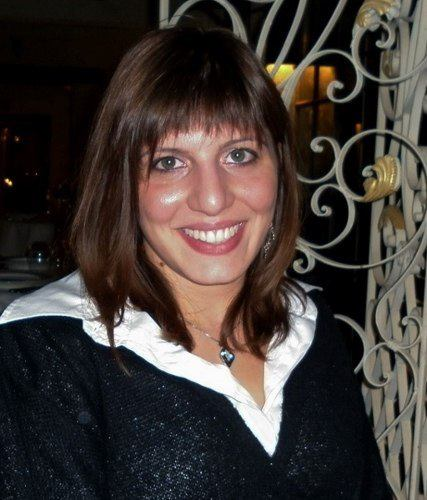
\includegraphics[scale = 0.6]{img/ale.jpg} &  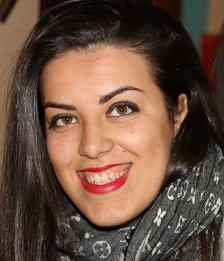
\includegraphics[scale = 0.6]{img/bea.jpg} & 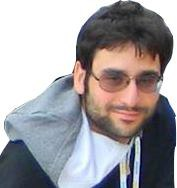
\includegraphics[scale = 0.6]{img/io.jpg} \\
  
  \hline
\end{tabular}


%%% \begin{itemize}
%%% \item Titolo di studio:\\ \\
%%% \item Interessi particolari:\\ \\
%%% \item Ha sostenuto fino ad oggi il seguente numero di esami:\\ \\
%%% \item Deve ancora sostenere i seguenti esami del I anno:\\ \\
%%% \item Prevede di svolgere un tirocinio presso:\\ \\
%%% \item Prevede di laurearsi nella sessione:\\ \\
%%% \item Intende proseguire gli studi per conseguire: \\  \\  \\
%%%   	presso la sede universitaria di: \\ \\
%%% \item Intende entrare subito nel mondo del lavoro presso : \\ \\
%%% \end{itemize}

 
\appendix


\bibliographystyle{abbrv}
\bibliography{biblio}

\end{document}